\documentclass{VUMIFPSkursinis}
\usepackage{algorithmicx}
\usepackage{algorithm}
\usepackage{algpseudocode}
\usepackage{amsfonts}
\usepackage{amsmath}
\usepackage{bm}
\usepackage{caption}
\usepackage{color}
\usepackage{float}
\usepackage{graphicx}
\usepackage{listings}
\usepackage{subfig}
\usepackage{wrapfig}

% Titulinio aprašas
\university{Vilniaus universitetas}
\faculty{Matematikos ir informatikos fakultetas}
\department{Programų sistemų katedra}
\papertype{Programų sistemų labaratorinis darbas}
\title{Stalo žaidimų programėlė}
\titleineng{Board games application}
\status{2 kurso 5 grupės studentai}
\author{Elena Reivitytė}
\secondauthor{Matas Šilinskas}
\thirdauthor{Kasparas Taminskas}
\fourthauthor{Aidas Vaikšnoras}
\fifthauthor{Tadas Žaliauskas}
\supervisor{dr. Vytautas Valaitis}
\date{Vilnius – \the\year}

% Nustatymai
% \setmainfont{Palemonas}   % Pakeisti teksto šriftą į Palemonas (turi būti įdiegtas sistemoje)
\bibliography{bibliografija}

\begin{document}
\maketitle

\tableofcontents

\sectionnonum{Įvadas}
Board games - tai aplikacija sujungianti norinčius žaisti stalo žaidimus žmones
su tais kuriems trūksta žaidėjų.

\section{Užduotys}
Pagrindinės sistemos užduotys ir su jomis susiję agentai

	\renewcommand{\labelitemi}{$\bullet$}
	\renewcommand{\labelitemii}{$\circ$}
	\begin{itemize}
		\item Agentai:
			\begin{description}
				\item [$\circ$ Svečias] Neprisijungęs programėlės naudotojas.
				\item [$\circ$ Registruotas vartotojas] Žmogus, sėkmingai atlikęs registraciją ir prisijungęs prie programėlės, galintis dalyvauti jos veikloje.
				\item [$\circ$ Žaidimo dalyvis] Registruotas vartotojas, nusprendęs prisijungti prie vieno iš sistemos siūlomų žaidimų.
				\item [$\circ$ Žaidimo šeimininkas] Registruotas vartotojas, pridėjęs žaidimą sistemoje.
				\item [$\circ$ Administratorius] Žmogus, atsakingas už tinkamą sistemos darbo palaikymą.
			\end{description}
	\end{itemize}
		
	\subsubsection*{Pagrindinės užduotys}
	
	\subsection{Svečio ir registruoto vartotojo užduotys}
		\begin{figure}[H]
			\centering
			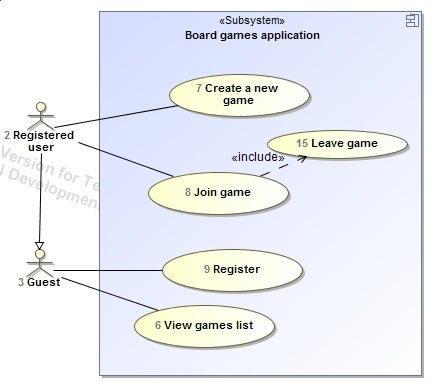
\includegraphics[scale=0.5]{img/UzduociuDiagrama1}
			\caption{Svečio ir registruoto vartotojo užduotys}
			\label{img:UzduociuDiagrama1}
		\end{figure}
		Kol vartotojas nėra užsiregistravęs sistemoje, jam suteikiamos tik svečio teisės, kurios leidžia tik peržiūrėti sukurtus žaidimus. Norėdamas įgyti daugiau privilegijų, vartotojas privalo užsiregistruoti. Registruotas vartotojas jau gali dalyvauti programėlės veikloje: sukurti naują žaidimą ir apie jį paskelbti, arba prisijungti prie jau esamo.

	\subsection{Žaidimo dalyvio ir šeimininko užduotys}
		\begin{figure}[H]
			\centering
			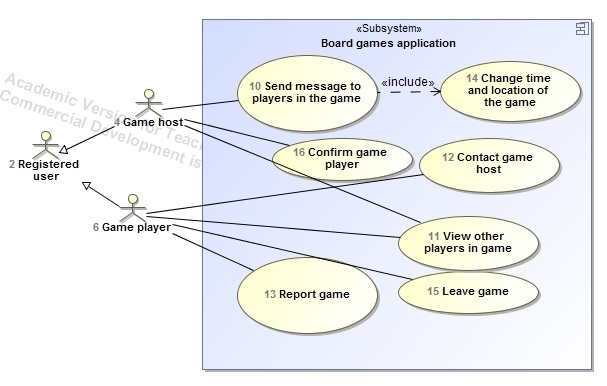
\includegraphics[scale=0.5]{img/UzduociuDiagrama2}
			\caption{Žaidimo dalyvio ir šeimininko užduotys}
			\label{img:UzduociuDiagrama2}
		\end{figure}
		Registruotas vartotojas gali atlikti du vaidmenis: arba būti sukurto žaidimo šeimininku, arba paprasčiausiu dalyviu. Žaidimo dalyviui leidžiama pranešti sistemos administratoriui apie nevykstantį žaidimą, tuo atveju, jeigu žaidėjas nuvyko į sutartą žaidimo vietą reikiamu laiku ir jam nepavyko surasti kitų užsiregistravusių dalyvių. Jeigu bent vienas žaidėjas (išskyrus šeimininką) nesutinka su tokia informacija, pranešimas laikomas melagingu. Priešingu atveju, sulaukus administratoriaus pritarimo, žaidimas išimamas iš aktyvių žaidimų sąrašo norint užkirsti tolimesnį galimą dalyvių pritraukimą. Tai pat, šeimininkui patvirtinus žaidėją, jis įgauna teisę peržiūrėti kitų, jau pareiškusių norą dalyvauti žaidėjų profilius ir su jais susipažinti naudojantis programėlės asmeninių žinučių sistema. Norėdamas pasiteirauti dėl žaidimo detalių arba visais kitais iškilusiais klausimais, jis taip pat gali tiesiogiai kreiptis į žaidimo šeimininką. Na o šeimininkas gali informuoti žaidėjus apie nenumatytai pasikeitusią žaidimo vietą ar laiką, susisiekti su jais ir iš anksto trumpai supažindinti su žaidimo taisyklėmis ir pnš. Jeigu žaidimo dalyviui nepatinka kitų dalyvių kompanija ar bet kokios kitos žaidimo detalės, jis gali bet kada palikti žaidimą, o žaidimo šeimininkas apie tai yra informuojamas.

	\subsection{Sistemos administravimas}
		\begin{figure}[H]
			\centering
			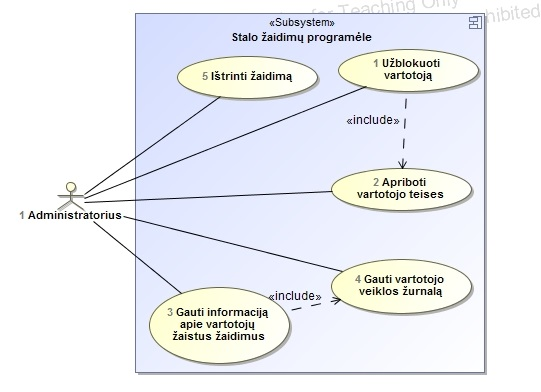
\includegraphics[scale=0.5]{img/UzduociuDiagrama3}
			\caption{Sistemos administravimas}
			\label{img:UzduociuDiagrama3}
		\end{figure}
		Administratorius prižiūri programėlės pateikiamos informacijos patikimumą. Jis turi teisę ištrinti registruoto vartotojo sukurtą žaidimą siekdamas apsaugoti dar vėliau prie žaidimo galimai prisijungsiančius dalyvius tuo atveju, jei vartotojo pateikti duomenys nėra tikslūs ar apie žaidimą jau buvo gautas įspėjamas pranešimas iš kitų sąžiningų vartotojų. Jeigu vartotojas nesiliauja kurti fiktyvių žaidimų, jam gali būti taikomos nuobaudos: laikinai (pvz. parai) apribojimas organizuoti bet kokius žaidimus. Jei tai kartojasi, administratorius gali apsvarstyti pasiūlymą užblokuoti vartotojo paskyrą arba įtraukti jo IP adresą į nepageidaujamų sąrašą. Kaip pagalbinę priemonę vartotojų veiksmams sekti administratorius gali naudoti vartotojų veiklos žurnalą, kuriame būtų pateikiami chronologiškai surikiuoti vartotojų veiksmai, gauti nurodžius dominantį periodą. Veiklos žurnalą būtų galima filtruoti pagal konkretų vartotoją, taip susiaurinant paiešką.		

\section{Procesų pjūvis}
Aplikacijoje yra vartotojo sąsajos, duomenų apdorojimo ir duomenu bazės procesai. 
Vartotojas tiesiogiai bendraudamas su vartotojo sąsaja, siunčia asinchronines 
žinutes duomenų apdorojimo procesui, kuris savo ruožtu bendrauja su duomenų baze.

	\subsection{Prisijungimas}
		\subsubsection*{Prisijungimo procesų sekos diagrama :}
		\begin{figure}[H]
			\centering
			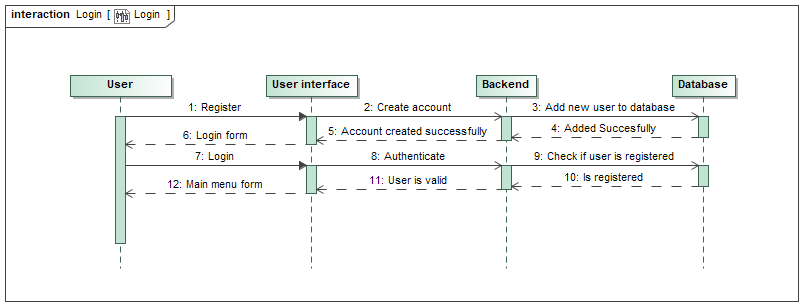
\includegraphics[scale=0.5]{img/Login_sequence}
			\caption{Prisijungimo procesų sekų diagrama}
			\label{img:MainWindow_activity}
		\end{figure}
		Visų pirma vartotojas privalo užsiregistruoti. Vartojo sąsaja nusiunčia JSON 
		žinutę su gautais duomenimis loginiam procesui, kuris patikrina ar duomenys yra tinkami ir
		prideda vartotoją į duomenų bazę. Užsiregistravęs vartotojas turi prisijungti,
		procedūra ganėtinai panaši - vartotojo sąsajoje gauti duomenys patikrinami ir 
		jei jie yra validūs, patikrinama ar slaptažodis sutampa su esančiu duomenų
		bazėje. Autentifikuotas vartotojas yra prijungiamas prie programėlės. 
		Jei slaptažodis netinka arba vartotojas nerastas duomenų bazėje, leidžiama
		patikslinti prisijungimo laukus ir prisijungimo procesas kartojamas dar kartą.

	\subsection{Pagrindinis navigacijos langas}
		\begin{figure}[H]
			\centering
			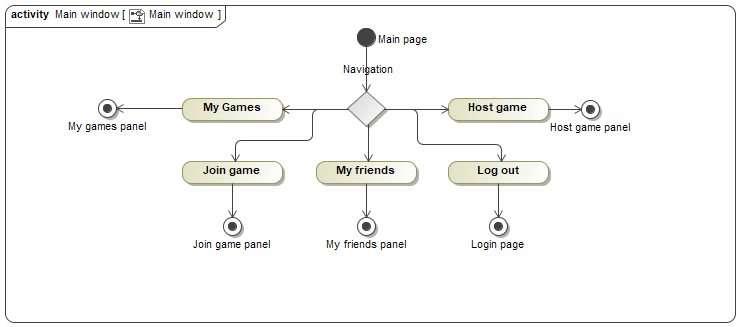
\includegraphics[scale=0.5]{img/MainWindow_activity}
			\caption{Pagrindinio navigacijos lango veiklos diagrama}
			\label{img:MainWindow_activity}
		\end{figure}
		\subsubsection*{Pagrindiniame navigacijos lange vartotojas paspaudęs atitinkamus mygtukus gali:}
			\renewcommand{\labelitemi}{$\bullet$}
			\begin{itemize}
				\item Atidaryti žaidimo sukūrimo langą.
				\item Atidaryti prisijungimo prie žaidimo langą.
				\item Atidaryti draugų sąrašo langą.
				\item Atidaryti mano žaidimų langą
				\item Atsijungti
			\end{itemize}

	\subsection{Žaidimo sukūrimo langas}
		\subsubsection*{Žaidimo sukūrimo veiklos diagrama :}
			\begin{figure}[H]
				\centering
				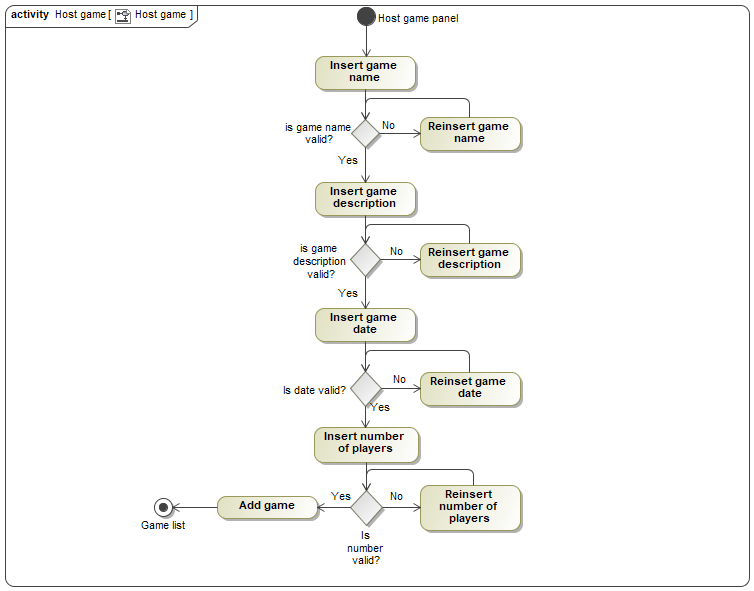
\includegraphics[scale=0.5]{img/HostGame_activity}
				\caption{Žaidimo sukūrimo veiklos diagrama}
				\label{img:Hostgame_activity}
			\end{figure}
			\subsubsubsection*{Žaidimo sukūrimo lange vartotojas turi įvesti :}
				\renewcommand{\labelitemi}{$\bullet$}
				\begin{itemize}
					\item Žaidimo pavadinimą.
					\item Žaidimo aprašymą.
					\item Žaidimo datą.
					\item Žaidėjų skaičių
				\end{itemize}
			Įvedimo metu tikrinama ar duomenys įvesti leistinu formatu. Jei formatas 
			netinkamas, vartotojas turi pataisyti atitinkamus duomenų laukus. Tinkamai
			užpildžius laukus,leidžiama pridėti žaidimą.
		\subsubsection*{Žaidimo sukūrimo procesų sekų diagrama :}
			\begin{figure}[H]
				\centering
				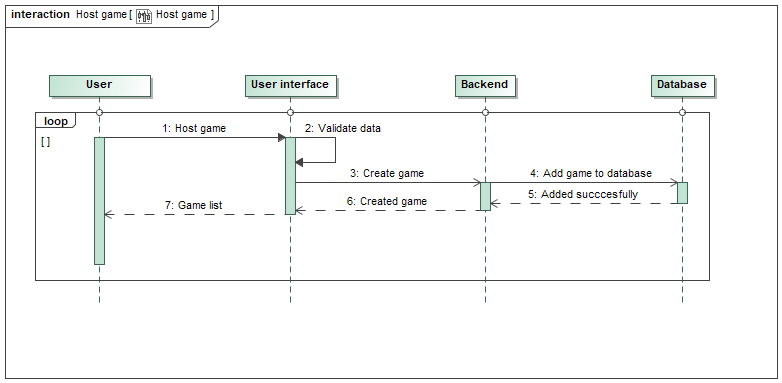
\includegraphics[scale=0.5]{img/HostGame_sequence}
				\caption{Žaidimo sukūrimo procesų sekų diagrama}
				\label{img:Hostgame_sequence}
			\end{figure}
			Vartotojas norėdamas sukurti žaidimą įveda žaidimo duomenis. Įvedimo metu 
			tikrinama ar duomenys įvesti leistinu formatu. Jei duomenys tinkami, tada 
			jie JSON formatu išsiunčiami loginiam procesui, kuris sukuria žaidimą ir 
			įrašo į duomenų bazę.	
			
	\subsection{Prisijungimo prie egzistuojančio žaidimo langas}	
		\subsubsection*{Prisijungimo prie egzistuojančio žaidimo veiklos diagrama :}
			\begin{figure}[H]
				\centering
				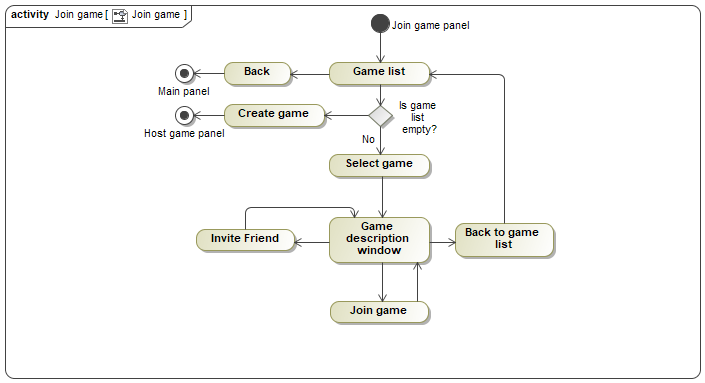
\includegraphics[scale=0.5]{img/JoinGame_activity}
				\caption{Prisijungimo prie egzistuojančio žaidimo veiklos diagrama}
				\label{img:JoinGame_activity}
			\end{figure}
			Iš pradžių vartotojui atidaromas egzistuojančių žaidimų sąrašas. Čia 
			vartotojas gali grįžti pagrindinį navigacijos langą arba tęsti žaidimo
			pasirinkimą. Jei nėra žaidimų prie kurių būtų galima prisijungti, vartotojui
			pasiūloma sukurti naują žaidimą. Vartotojui sutikus jis nukreipiamas į 
			žaidimo sukūrimo langą. Jei žaidimų sąrašas nėra tučias, tai vartotojas
			gali pasirinkti žaidimą prie kurio norėtų prisijungti. Pasirinkus atidaromas
			pasirinkto žaidimo aprašymo langas. Čia vartotojas gali pakviesti draugus
			kartu žaisti pasirinktą žaidimą, pats prisijungti prie žaidimo arba grįžti
			atgal į žaidimų sąrašą ir pasirinkti kitą žaidimą.
		\subsubsection*{Prisijungimo prie egzistuojančio žaidimo sekų diagrama :}
			\begin{figure}[H]
				\centering
				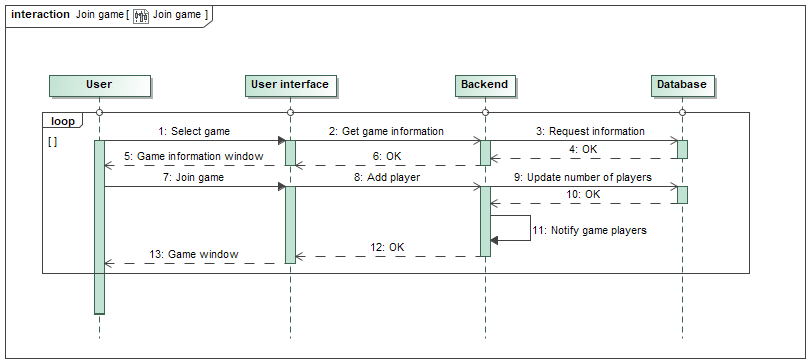
\includegraphics[scale=0.5]{img/JoinGame_sequence}
				\caption{Prisijungimo prie egzistuojančio žaidimo procesų sekų diagrama}
				\label{img:Hostgame_sequence}
			\end{figure}
			Žaidėjui pasirinkus žaidimą iš sąrašo, atidaromas žaidimo informacijos 
			langas. Informaciją apie žaidimą suteikia logikos procesas, kuris
			nusiuntęs užklausą į duomenų bazę, gauna papildomą informaciją apie 
			pasirinktą žaidimą. Vartotojui nusprendus prisijungti prie žaidimo, 
			nusiunčiama žinutė atnaujinti prisijungusių žaidėjų skaičių duomenų bazėje,
			taip pat visiems tame žaidime užsiregistravusiems žaidėjams išsiunčiamas 
			pranešimas apie naują prisijungusį žaidėją.

	\subsection{Draugų sąrašo langas}		
		\subsubsection*{Draugų sarašo lango sekų diagrama :}
			\begin{figure}[H]
				\centering
				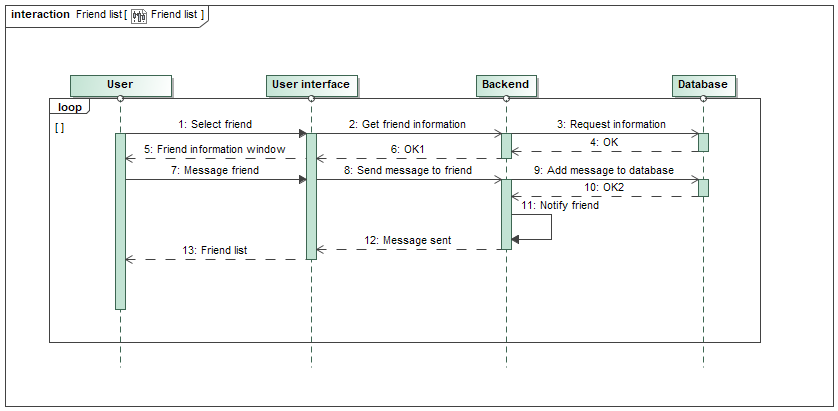
\includegraphics[scale=0.5]{img/FriendList_sequence}
				\caption{Draugų sarašo lango sekų diagrama}
				\label{img:FriendList_sequence}
			\end{figure}
			Vartotojui pasirinkus draugą iš draugų sąrašo, paprašoma loginio proceso
			gauti daugiau duomenų apie draugą iš duomenų bazės. Tuomet atidaromas 
			langas su daugiau duomenų apie draugą. Paspaudus siųsti žinutę logikos 
			procesas išsaugo žinutę duomenų bazėje ir praneša draugui apie gautą žinutę.
			
	\subsection{Žaidimo langas}		
		\subsubsection*{Žaidimo lango sekų diagrama :}
			\begin{figure}[H]
				\centering
				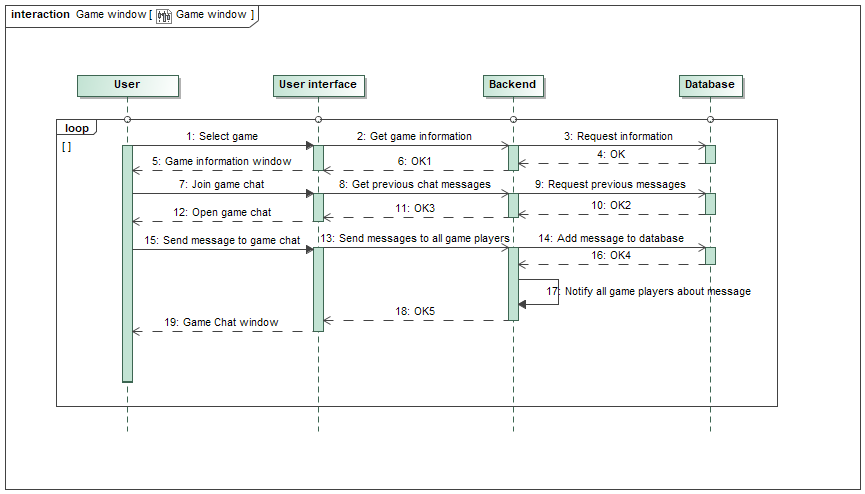
\includegraphics[scale=0.5]{img/GameWindow_sequence}
				\caption{Žaidimo lango sekų diagrama}
				\label{img:GameWindow_sequence}
			\end{figure}
			Vartotojui pasirinkus žaidimą iš žaidimų sąrašo, paprašoma loginio proceso
			gauti daugiau duomenų apie žaidimą iš duomenų bazės. Tuomet atidaromas 
			langas su daugiau duomenų apie žaidimą. Paspaudus siųsti žinutę logikos 
			procesas paprašo žaidimo susirašinėjimo istorijos iš duomenų bazės. Tada
			atidaromas pokalbių langas, kur vartotojas gali išsiųsti žinutę visiems 
			prie žaidimo prisijungusiems žaidėjams. Paspaudus siųsti žinutę logikos 
			procesas išsaugo žinutę duomenų bazėje ir praneša žaidėjams apie gautą žinutę.

\end{document}
